\section{Overview}
In this section we will provide a high-level view and description of the components that our system is made of. The architecture chosen for our system is a three-tier one. The major advantages of this architectural style is the decoupling of the application logic from the presentation logic and the data persistence concerns. Further details about the characteristics of this architectural style will be given in section 2.6, for now we will proceed with the general overview of the system. In the picture below is illustrated a high-level view of the system with an informal notation, where each rectangular box represents a high-level computational unit of the system, meanwhile the double-edged arrow represents 
 the interaction between two components. \\
\begin{figure}[H]
    \centering
    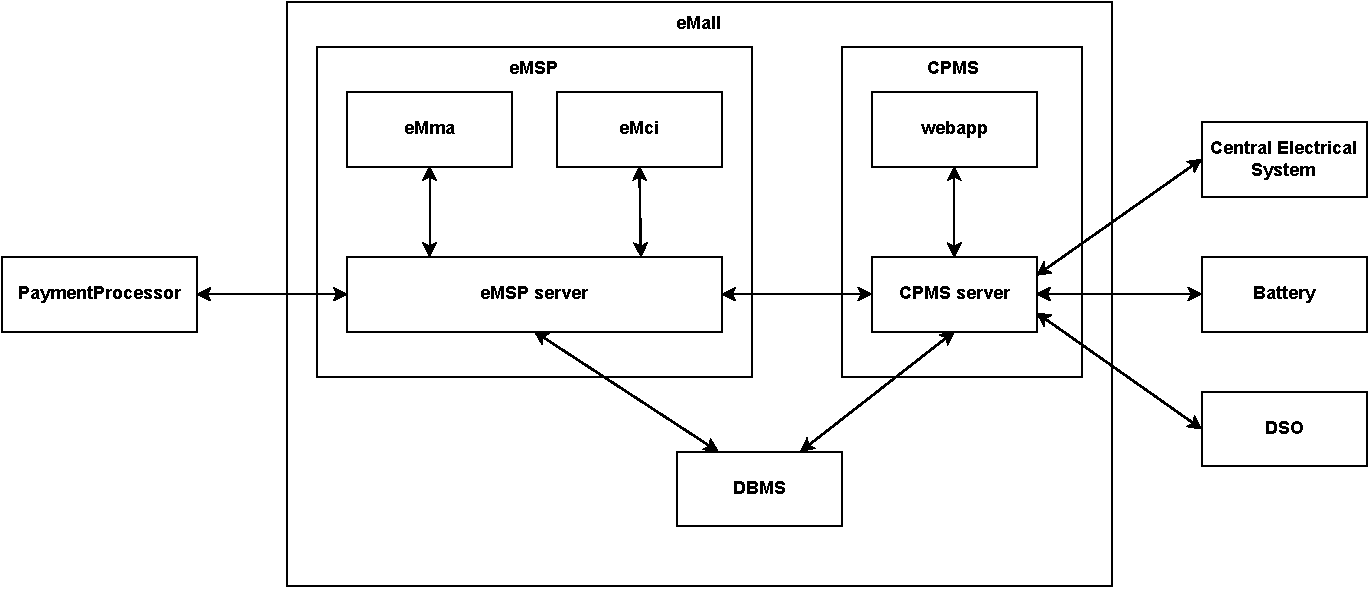
\includegraphics[width=0.8\textwidth]{Images/cp2/overview.pdf}
    \caption{High level description of the components and their interactions}
\end{figure}

\par
%TODO: Bianca please check if you can understand this pargarph
The eMall system, illustrated in the figure, is the objective of this design document. It is clear that the system is divided in two main sub-systems: eMSP and CPMS. This choice is driven by an interoperability requirement of the eMSP and the CPMS with different CPMS and eMSP systems respectively, offered by other companies. Nonetheless, this low-coupling of the CPMS with the eMSP doesn't preclude us from reusing components that have the same functionality in both sub-systems. It is also important to point out that our system, specifically the CPMS sub-system, must be able to interface with the system responsible for managing the technical aspect of the charging point, the system that manages the battery, if present, and the DSO's software system.
\par
As we stated previously, the system has a three-tier architecture. In particular the three tiers are:

\paragraph{Client tier} It's the tier closest to the user and its duty is to manage the user interaction. This means that it must handle the visualization of the content to the user and interpret and translate the user interaction in requests to be forwarded to the application tier. We'd like to remark that this tier doesn't contain any application (or business) logic. We will use a client-side rendering software architecture to design this layer.

\paragraph{Application tier} This is the part where the core and the business logic of the system is implemented, consequently, this second layer realizes the functionalities required to the system, like the booking service or the charging station management service for the CPO. All this functionalities shall be discussed in more detail in the upcoming sections. As we will see in the following section, a micro-services approach has been used to build such layer.

\paragraph{Data tier} The third, and bottom tier, of our system is the data tier, where the persistence concerns of our system are met. The eMall system, both CPMS and eMSP sub-systems, has to handle a large amount of data, which must be carefully stored in order to have a properly working system. The data management is an aspect of software systems that has been thoroughly studied and developed, so the obvious choice for our system is to use an already implemented and tested Database Management System (DBMS).

\section{Component view}
In this section we will discuss and elaborate on the components that compose our system in order to implement the functionalities listed in the RASD document. We will start from a higher level of abstraction to provide a grasp of how the system works, thus even those who are not familiar with the technical aspect of a software system can understand at high level how the system is structured. Afterwards, we will proceed to further analyze the system at finer levels.
\begin{figure}[H]
    \centering
    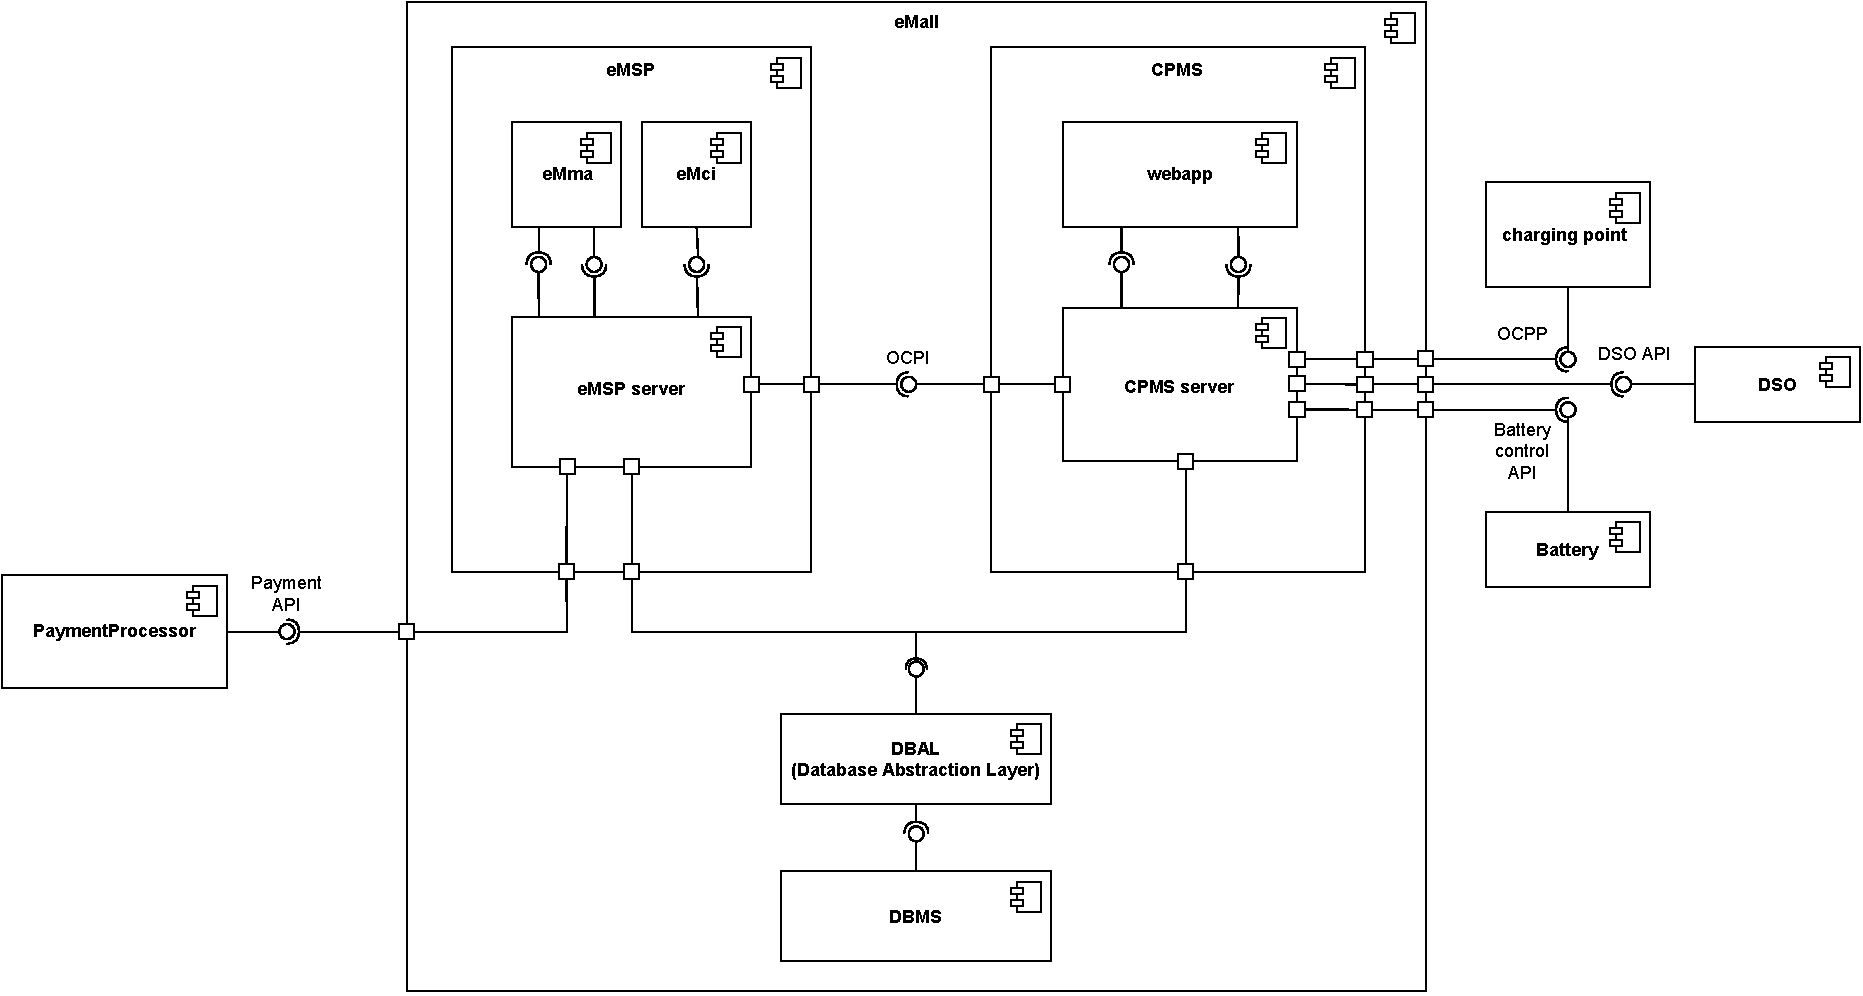
\includegraphics[width=1\textwidth]{Images/cp2/component_overview.pdf}
    \caption{Component view of the system}
\end{figure}

This component diagram provides a higher level view of how the system it is composed. It distinguishes the parts that the development team bust build (the eMall component), and lists the external system with their respective interfaces with which the eMall must interact to provide its functionalities. Furthermore, it's apparent that the system is composed by two main sub-systems, the eMSP and CPMS, that must interact with each other through the OCPI interface, and each of this sub-system is structured in a client-server architecture. The OCPI interface is an open and free interface that standardizes the interface of a CPMS, in other words it standardizes the services a CPSM offers and how to make request for these services to the CPMS. As a consequence of using the OCPI protocol we allow our eMSP to be able to interact with different CPMS\textit{s}, and our CPMS to interact with different eMSP\textit{s}, as per requirement. Finally, there are the DBMS and DBAL components, that compose the third and bottom tier of our architecture. The presence of the DBAL component tells us that a level of indirection from the DBMS has been added, allowing the system to be independent from any particular DBMS.
\par
In the next paragraphs we shall discuss in more detail the composite structure of the main sub-systems of the eMall: the eMSP and CPMS.
\pagebreak

\textbf{eMSP}\\
\begin{figure}[H]
    \centering
    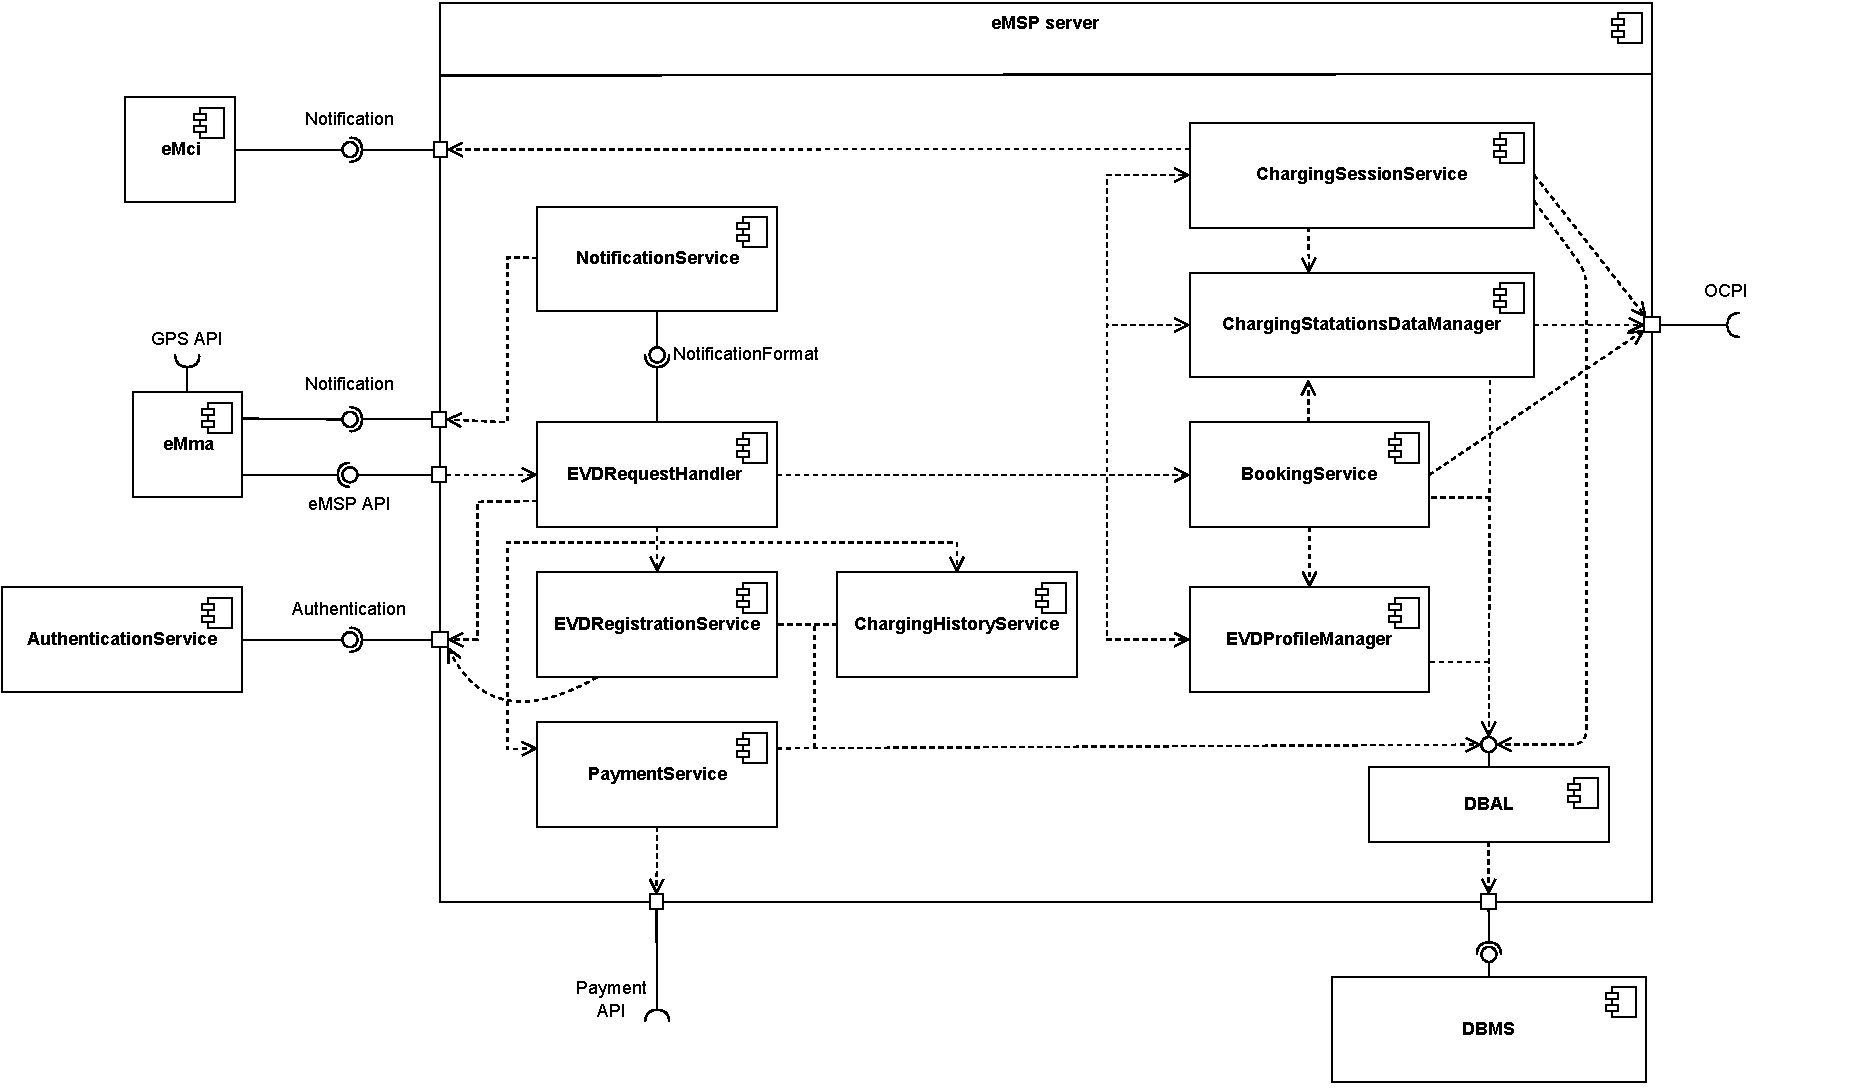
\includegraphics[width=1\textwidth]{Images/cp2/eMSP_server.pdf}
    \caption{eMSP composite structure}
\end{figure}

The eMSP is the system that will interact with the EVD and forward his charging request to the CPMS. As we can see the eMSP isn't only a middleman between the EVD and the CPMS but offers other services like profile management, payment services and charging history services. Below we provide a brief description of each component of the eMSP:
\begin{itemize}
    \item \textbf{eMma}: eMall mobile app. It is the client componet of the eMSP, its task si to act as a view and controller for the EVD interactions. Specifically, it will provide a GUI to the user from which he can make his request to the eMSP. Furthermore it will encode the user input and interaction with the view to the corresponding functions of the eMSP server interface. Finally it has to interact with the GPS module of the OS in which it will run to provide location information to the eMSP
    
    \item \textbf{eMci}: eMall charging interface. This component's role is to provide the graphical interface the EVD will be using at the charging point when he wants to start a charging session and is located on an embedded device on the charging point. It's job is then to identify the charging point in which it resides so the EVD can inform the eMSP of which charging point he wants to use

    \item \textbf{DBMS}: Database Management Service. It is the usual system with the task of managing the insertion, storing, deletion and update of the data generated by the system. This component exceptionally complex and given the widely availability of this kind on systems on the market, using an already build and thoroughly tested one will be mandatory

    \item \textbf{DBAL}: Database Abstraction Layer. It functions as an additional layer of indirection form the DBMS. In this manner the eMSP will be independent of the DBMS used and if this component changes in the future the eMSP won't need to be modified to integrate the interface of the new DBMS

    \item \textbf{AuthenticationService}: Component that has to mange user's authentication to the system and authorization to use the services

    \item \textbf{PaymentService}: This component, through the usage of external Payment API offered by external providers, allows the eMSP to handle the payment requests from the users

    \item \textbf{ChargingHistoryService}: The component which has to process the data saved in the DB to present the user with a functional information regarding his charging history

    \item \textbf{EVDRegistrationService}: Component which has to handle the user registration process. Obviously it shall use the the DBAL to store the user information once the process has finished. Additionally it also has to use the component AuthorizationService in order to login the user once the registration process has successfully ended

    \item \textbf{EVDProfileManager}: Component responsible for managing and processing the data concerning the EVD personal information and the EVD's data about his EVs

    \item \textbf{ChargingStationsDataManager}: This is one of the main components of the system. It has to interact with the CPMS to gather data useful for the EVD and more specifically that will be used and processed by the other components. Moreover it acts as an interface for other components that need information about the stations, so don't need to depend on the data structure used to store the stations

    \item \textbf{ChargingSessionService}: Component responsible for unlocking the charging point, starting the charging session and terminating it. Obviously to offer this services it must interact with the CPMS trough the OCPI interface. Additionally it uses the DBAL interface in order to save the data about the charging session, which will be used by the ChargingHistoryService component, and can perform checks when the user is trying to unlock the wrong charging point by cross-checking the data stored in the DB about the charging points and the code it receives by the eMci component

    \item \textbf{BookingService}: Component that provides the booking functionality. It must use the EVDProfileManger and the ChargingStationsDataManager components to get the specific information about the user and the station respectively in order to make the appropriate request through the OCPI interface. Moreover it stores this information in the DB so that when can be used to cancel a booking
    %TODO: if the OCPI doesn't allow to cancel a booking and allows only booking within 15 min what we do, we have to change requirements and functionalities. Or we can accept the booking, wai and try booking through the CPMS when the time comes (needs to send notification if it doesn't succeed).
    
    \item \textbf{NotificationService}: Component that provides the eMSP server with the capability of sending notification to the EVD through the eMma component, consequently this component must use the communication interface offered by eMma

    \item \textbf{EVDRequestHandler}: All the users' requests pass trough this component. This centralized approach is need so the system can check if the requests have the right permissions (i.e. request for services allowd only for registered user). This explains the dependency with the AuthenticationService component. Obvioulsy it also need to use all the other components to grant the user the services offered by the system

\end{itemize}
\pagebreak

\textbf{CPMS}\\
\begin{figure}[H]
    \centering
    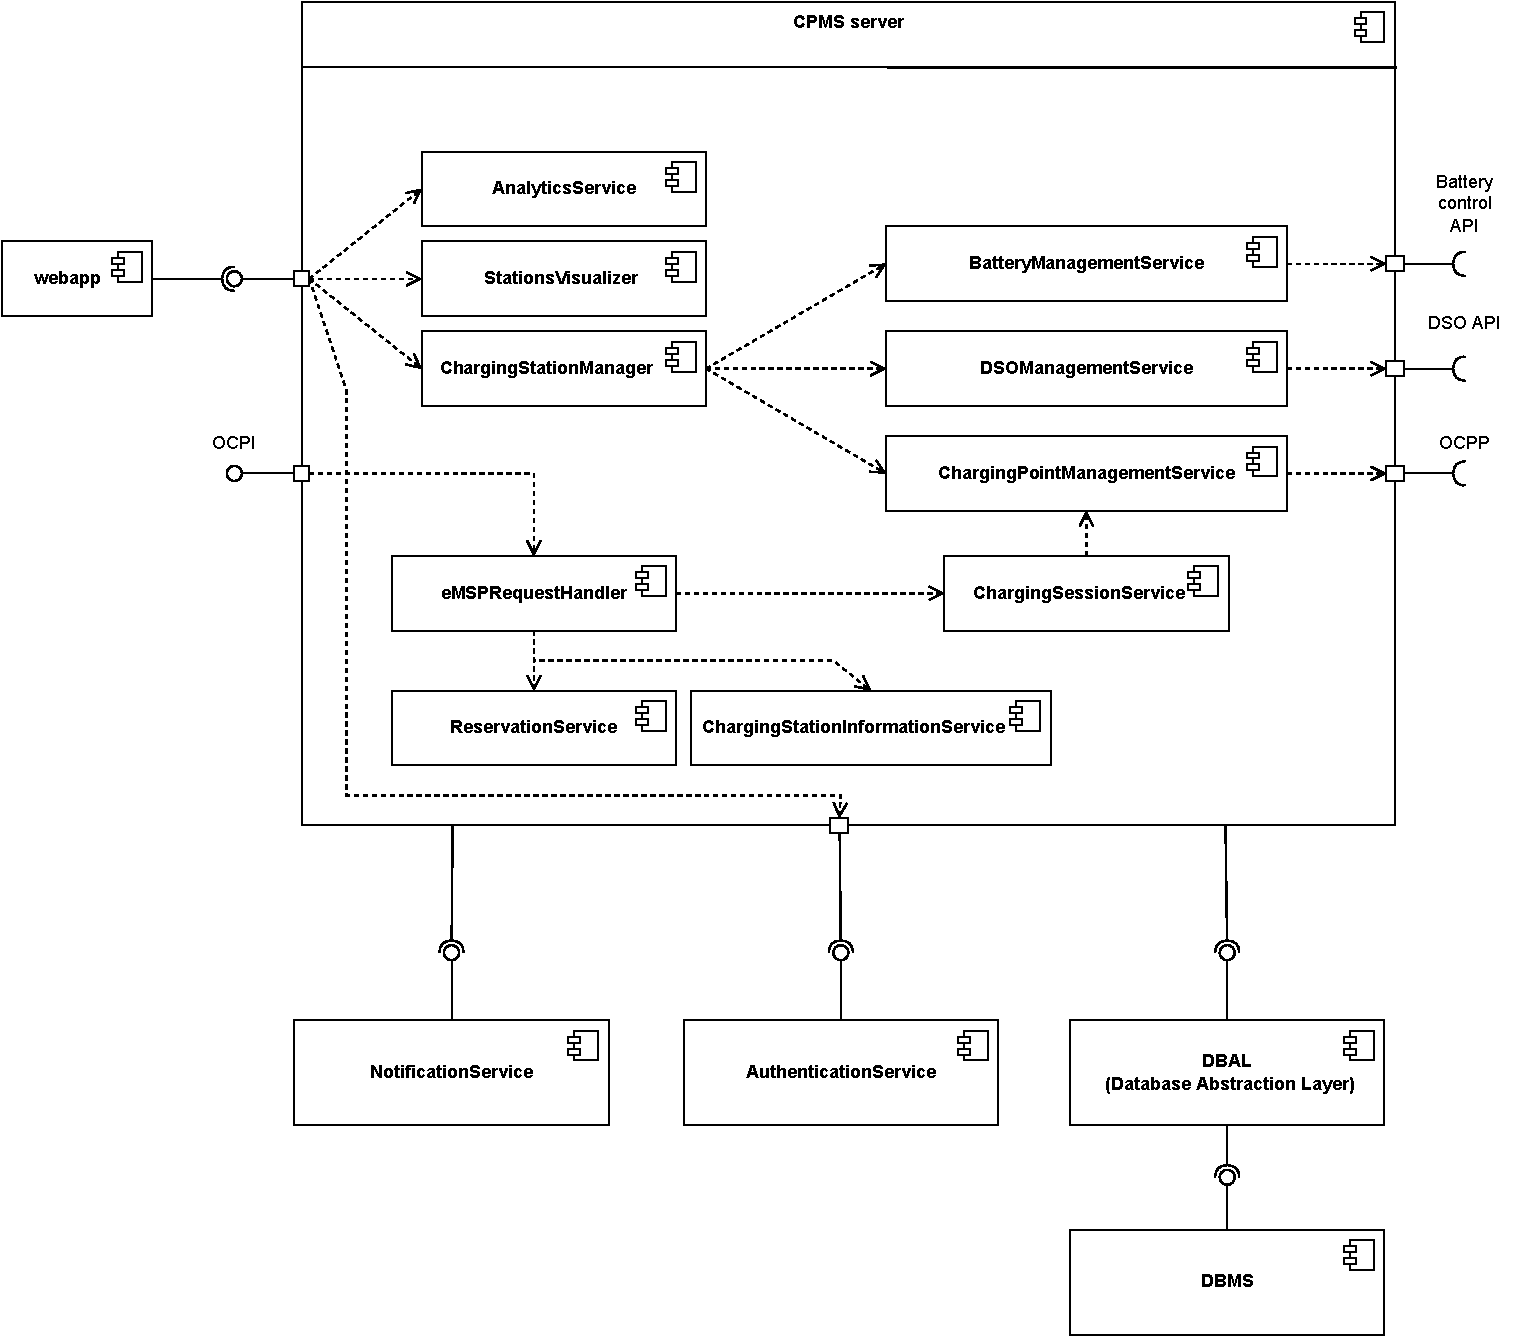
\includegraphics[width=1\textwidth]{Images/cp2/CPMS_server.pdf}
    \caption{CPMS composite structure}
\end{figure}

The CPMS is the subsystem responsible for manging the charging station, offering charging services to EVDs and securing the electricity supply from the DSOs. To offer all this functionalities this sub-system of the eMall must collaborate with other systems external to our own, which can be viewd in the general overview. Specifically, the CPMS needs to interfaces to the system responsible of managing the battery by the \verb|Battery control API| interface, with the DSO IT system through it's API and with the the system managing the charging points devices through the protocol OCPP, which is an open standard. Like we have done for the eMSP, we will proceed describing each component of the CPMS sub-system (components AuthenticationService, DBAL, DMBS and NotificationService have the same functionality as in the eMSP system and shall not be repeated here):

\begin{itemize}
    \item \textbf{ChargingPointManagmentService}: Component responsible for interacting with the central management system of charging station. This component will query this central system through the OCPP protocol, asking for the status of the charging points, and invoking request like starting (likewise terminating) the flow of electricity of a particular charging point to start a charging session

    \item \textbf{DSOManagementService}: Component responsible for collecting the data from the various DSO and concluding sales contracts with them if the API allows it

    \item \textbf{BatteryManagementService}: Component responsible for managing the battery of the charging station if one is present. This component must interface with the software system managing the technical aspects of the battery trough its control API (here called Battery control API) and must use the methods provided by the ChargingPointManagemntService component to allow the central system to switch to the battery for charging or charging the battery when requested

    \item \textbf{StationsVisualizer}: Component that allows the CPO to visualize and select one of the charging stations managed by him

    \item \textbf{AnalyticsService}: Component that provides the CPO with the tools to do some statistical analysis on the data collected by each charging station

    \item \textbf{ChargingStationManager}: Main component responsible for the interaction with the CPO. It implements all the functionalities related to the business aspect of the charging station (setting electricity price, promotions, etc.) and uses the component described before for managing the technical aspects of the charging station. This component also uses the NotificaionService component to notify the CPO about any necessary information

    \item \textbf{CPORequestHandler}: It is the component where all the CPO request must first pass trough in order to perform security checks and allow only authorized user to access the services of the CPMS. To offer this functionality the component makes use of the AuthenticationService component to login the user and to check if the request coming from the webapp have the necessary authorization. If a request passes the controls it's forwarded to the respective component

    \item \textbf{ChargingSessionService}: Component responsible for handling the starting, monitoring and terminating of a charging process

    \item \textbf{ChargingStationInformationService}: Component in charge of processing the data of the charging station, stored in the DB, in a suitable format for the eMSP and compatible with the OCPI interface

    \item \textbf{ReservationService}: Component responsible of managing the reservation of the charging points 

\end{itemize}

\section{Deployment view}
\begin{figure}[H]
    \centering
    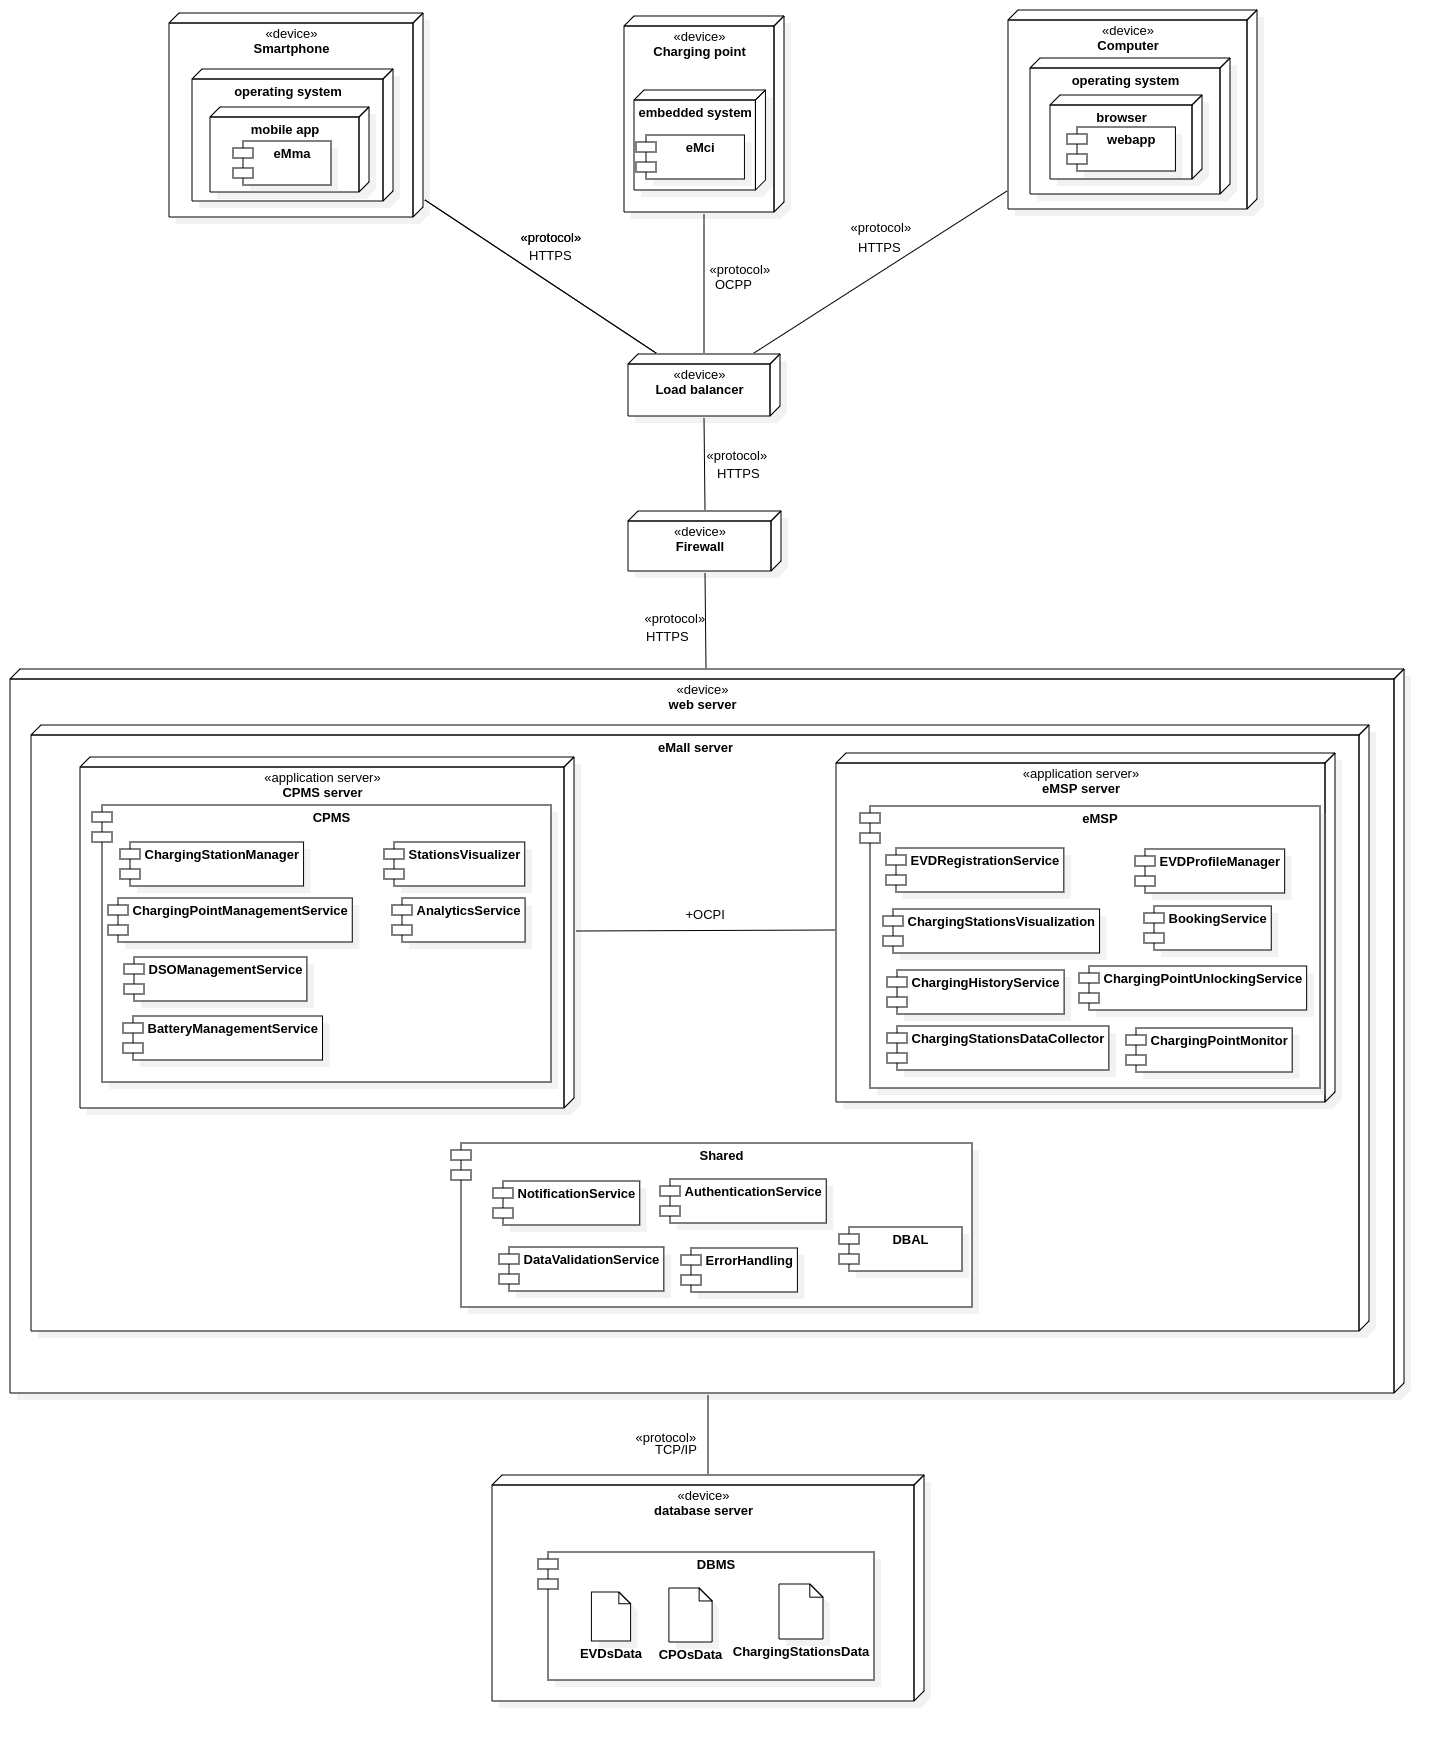
\includegraphics[width=1\textwidth, height=0.9\textheight]{Images/cp2/DeploymentDiagram.png}
    \caption{Deployment view of the system}
\end{figure}
At the client level we can see three different devices interacting with the system:
\begin{itemize}
    \item \textbf{Smartphone} - The smartphone runs the mobile application of the eMall, the eMma, and has internet access in order to send the HTTPS requests to the system. This is the kind of device used by the EVDs that use the eMall
    \item \textbf{Computer} - The computer runs the web application of the eMall, and also has internet access to manage the service through HTTPS requests to the system. This is the kind of device used by the CPOs of the companies that use the eMall to manage their charging stations
    \item \textbf{Charging Point} - The charging point is the specific device used by the EVDs to charge the EVs and it has an embedded system, which through the OCPP protocol communicates with the CPMS part of the eMall system, in order to correctly provide the charging service
\end{itemize}

Between the client level and the application level, we have some architectural elements that allow to achieve some non-functional requirements, such as better performance, scalability, availability and security:
\begin{itemize}
    \item \textbf{Load balancer} - The load balancer is a network device that distributes incoming requests across a group of servers to help improve the performance and availability of the application. A load balancer can help to improve the performance of the application by distributing incoming requests across multiple servers, rather than routing all requests to a single server. This can help to prevent any single server from becoming overloaded, which can improve the overall responsiveness and performance of the application. A load balancer can make it easier to scale the application horizontally by allowing to add or remove servers as needed and this can be useful if we need to add more capacity to handle a growing number of users. A load balancer can, also, help to improve the availability of the application by routing traffic to a healthy server in the event that one of the servers becomes unavailable. We can see that the load balancer is useful to improve different non-functional requirements of the eMall, that can be implemented using different servers to have better characteristics 
    \item \textbf{Firewall} - The firewall allows to protect the network from external threats and unauthorized access, blocking incoming traffic that does not meet the security rules. The firewall is necessary in order to comply with certain regulations and industry standards, because we are handling sensitive data (financial information, personal data), so is necessary to protect the data. The firewall can also help to improve the performance of the application by blocking traffic that is not necessary or relevant to the application, improving the overall responsiveness of the eMall
\end{itemize}

The eMall web application and mobile application provide both static and dynamically generated content, so the system runs web servers for the static content and application servers to generate content dynamically. The load balancer sends to the web server the HTTPS requests that need only static content, and on the other side sends to the correct application server the requests to generate the dynamic content and accomplish more complex functionalities due to the interaction of the eMall components. 
At the application level the deployment diagram shows in a simplistic way the following elements:
\begin{itemize}
    \item \textbf{Web server} - For the web server we have a computer that stores software and website raw data, such as HTML files, images, text documents, and JavaScript files. The hardware of the web server is connected to the web and supports the data exchange with different devices connected to the Internet
    \item \textbf{Application server} - In the deployment diagram on the same hardware we also have the application servers, one for the CPMS and one for the eMSP, with also the shared services. The application servers contain different micro-services, that interact among them and with external APIs, as shown in the previous component diagram. The micro-services could also be implemented on more servers, splitting the eMSP and CPMS application servers in more servers, or creating a redundancy of the available services on different machines to improve performance and availability, exploiting even better the load balancer
    \item \textbf{Shared components} - The shared components shown in the diagram are components that belong to the two application servers, but also to the web server. The web server of the eMall handles part of these functionalities, sending the rest to the application servers  
\end{itemize}

Finally at the lowest level we have the persistent part of the system, which interacts with the eMall trough TCP/IP and is hidden to the higher levels due to the use of the DBAL. The Database level is composed by:
\begin{itemize}
    \item \textbf{Database server} - It hosts the database of the system and manages the different data through a DBMS 
    \item \textbf{Database artifacts} - The different database artifacts shown in the diagram represent physical implementations of the DB, an implementation for the data regarding the EVDs, one for the companies and CPOs data and finally an implementation for the data regarding the charging stations and any other related data
\end{itemize}
For a more secure system we consider not only a DB, but also some replicas, distributed on different machines to guarantee more availability, fault tolerance and disaster recovery. 

\section{Runtime view}

\section{Component interfaces}

\section{Selected architectural styles and patterns}

\section{Other design decisions}
